\chapter{Low-Density Parity-Check (LDPC) Codes}
\label{ch:ldpc}

\begin{nontechnical}
\textbf{LDPC codes are like a super-smart spell-checker that can fix corruption even when 40\% of letters are garbled}---and they're so good, they're in your WiFi, 5G phone, and satellite TV!

\textbf{The magic:}
\begin{itemize}
\item Regular error correction: Can fix maybe 10--20\% errors
\item LDPC: Can fix 40\%+ errors and get to near-theoretical limit!
\item How: Uses ``belief propagation''---bits check each other iteratively
\end{itemize}

\textbf{Real-world analogy---Sudoku:} Each bit is connected to multiple parity checks. Like sudoku: each number constrains others. Even if some numbers are missing, you can solve for them! LDPC does this with thousands of interconnected checks.

\textbf{Why they're everywhere:} WiFi 5/6, 5G phones, satellite TV (DVB-S2), deep-space probes, and SSDs all use LDPC codes. Within 0.5~dB of Shannon's theoretical limit!

\textbf{Fun fact:} LDPC codes were forgotten for 30 years because computers in the 1960s couldn't run the decoder in real-time. Today, your WiFi chip decodes LDPC billions of times per second without breaking a sweat!
\end{nontechnical}

\section{Overview}

\textbf{Low-Density Parity-Check (LDPC)} codes are a class of linear block codes used for forward error correction in modern communication systems. First invented by Robert Gallager at MIT in 1962, LDPC codes were rediscovered in 1996 and have since become the dominant coding scheme in many applications.

\begin{keyconcept}
LDPC codes achieve \textbf{near-Shannon-limit performance}, operating within 0.5~dB of the theoretical capacity limit for AWGN channels. This makes them one of the most powerful practical error correction codes available.
\end{keyconcept}

LDPC codes are characterized by their sparse parity-check matrix $\mathbf{H}$, where most entries are zero (hence ``low-density''). This sparsity enables efficient iterative decoding using belief propagation algorithms, making LDPC codes practical for high-speed implementations.

\section{Mathematical Description}

\subsection{Parity-Check Matrix}

An LDPC code is defined by an $m \times n$ sparse binary parity-check matrix $\mathbf{H}$:
\begin{equation}
\mathbf{H} = \begin{bmatrix}
h_{11} & h_{12} & \cdots & h_{1n} \\
h_{21} & h_{22} & \cdots & h_{2n} \\
\vdots & \vdots & \ddots & \vdots \\
h_{m1} & h_{m2} & \cdots & h_{mn}
\end{bmatrix}
\end{equation}
where:
\begin{itemize}
\item $h_{ij} \in \{0, 1\}$ = matrix elements
\item $m$ = number of parity check equations (rows)
\item $n$ = codeword length (columns)
\item Most entries are $0$ (low-density property)
\end{itemize}

\textbf{Example:} A $(7,4)$ LDPC code with $m=3$ parity checks and $n=7$ codeword bits:
\begin{equation}
\mathbf{H} = \begin{bmatrix}
1 & 1 & 0 & 1 & 1 & 0 & 0 \\
0 & 1 & 1 & 1 & 0 & 1 & 0 \\
1 & 0 & 1 & 0 & 0 & 0 & 1
\end{bmatrix}
\end{equation}

\subsection{Code Definition}

A valid LDPC codeword $\mathbf{c} = [c_1, c_2, \ldots, c_n]$ must satisfy:
\begin{equation}
\mathbf{H} \mathbf{c}^T = \mathbf{0} \pmod{2}
\end{equation}
where:
\begin{itemize}
\item $\mathbf{c}$ = transmitted codeword (length $n$ bits)
\item $\mathbf{0}$ = all-zero vector (length $m$ bits)
\item All arithmetic is modulo-2 (XOR operations)
\end{itemize}

\subsection{Code Rate}

The code rate defines the fraction of information bits to total bits:
\begin{equation}
R = \frac{k}{n} = \frac{n - m}{n}
\end{equation}
where:
\begin{itemize}
\item $k$ = number of information bits
\item $n$ = total codeword length
\item $m$ = number of parity checks
\item For the $(7,4)$ example: $R = 4/7 \approx 0.57$
\end{itemize}

\begin{calloutbox}{Common Code Rates}
Modern systems use standardized rates:
\begin{itemize}
\item $R = 1/2$: Strong error correction (50\% overhead)
\item $R = 2/3$: Balanced performance (33\% overhead)
\item $R = 3/4$: High efficiency (25\% overhead)
\item $R = 5/6$: Maximum throughput (17\% overhead)
\end{itemize}
Higher rates give more throughput but less error correction capability.
\end{calloutbox}

\subsection{Encoding Process}

For systematic encoding, the codeword structure is:
\begin{equation}
\mathbf{c} = [\mathbf{u} | \mathbf{p}]
\end{equation}
where:
\begin{itemize}
\item $\mathbf{u}$ = information bits (length $k$)
\item $\mathbf{p}$ = parity bits (length $m = n - k$)
\item Parity bits computed from $\mathbf{H}\mathbf{c}^T = \mathbf{0}$
\end{itemize}

The parity bits are calculated using:
\begin{equation}
\mathbf{p} = (\mathbf{H}_p^{-1} \mathbf{H}_u) \mathbf{u}^T
\end{equation}
where:
\begin{itemize}
\item $\mathbf{H}_u$ = submatrix corresponding to information bits
\item $\mathbf{H}_p$ = submatrix corresponding to parity bits (must be invertible)
\end{itemize}

\subsection{Tanner Graph Representation}

LDPC codes can be visualized as a bipartite graph with two types of nodes:

\begin{center}
\begin{tikzpicture}[scale=1.2]
% Variable nodes (circles)
\foreach \x in {0,1.2,2.4,3.6,4.8,6.0,7.2}
  \node[circle,draw,fill=white,minimum size=8mm,font=\small] (v\x) at (\x,0) {};

% Labels for variable nodes
\node[below=3pt,font=\scriptsize] at (0,-0.4) {$c_1$};
\node[below=3pt,font=\scriptsize] at (1.2,-0.4) {$c_2$};
\node[below=3pt,font=\scriptsize] at (2.4,-0.4) {$c_3$};
\node[below=3pt,font=\scriptsize] at (3.6,-0.4) {$c_4$};
\node[below=3pt,font=\scriptsize] at (4.8,-0.4) {$c_5$};
\node[below=3pt,font=\scriptsize] at (6.0,-0.4) {$c_6$};
\node[below=3pt,font=\scriptsize] at (7.2,-0.4) {$c_7$};

% Check nodes (squares)
\node[rectangle,draw,fill=black!10,minimum size=8mm,font=\small] (c1) at (1.5,2.5) {};
\node[rectangle,draw,fill=black!10,minimum size=8mm,font=\small] (c2) at (3.6,2.5) {};
\node[rectangle,draw,fill=black!10,minimum size=8mm,font=\small] (c3) at (5.7,2.5) {};

% Labels for check nodes
\node[above=3pt,font=\scriptsize] at (1.5,2.9) {$f_1$};
\node[above=3pt,font=\scriptsize] at (3.6,2.9) {$f_2$};
\node[above=3pt,font=\scriptsize] at (5.7,2.9) {$f_3$};

% Edges based on parity check matrix
% Check 1: bits 1,2,4,5
\draw[thick] (v0) -- (c1);
\draw[thick] (v1.2) -- (c1);
\draw[thick] (v3.6) -- (c1);
\draw[thick] (v4.8) -- (c1);

% Check 2: bits 2,3,4,6
\draw[thick] (v1.2) -- (c2);
\draw[thick] (v2.4) -- (c2);
\draw[thick] (v3.6) -- (c2);
\draw[thick] (v6.0) -- (c2);

% Check 3: bits 1,3,7
\draw[thick] (v0) -- (c3);
\draw[thick] (v2.4) -- (c3);
\draw[thick] (v7.2) -- (c3);

% Legend
\node[font=\small,align=left] at (9.5,1.8) {Variable nodes};
\node[font=\small,align=left] at (9.5,1.3) {(codeword bits)};
\node[circle,draw,fill=white,minimum size=6mm] at (8.3,1.55) {};

\node[font=\small,align=left] at (9.5,0.5) {Check nodes};
\node[font=\small,align=left] at (9.5,0.0) {(parity checks)};
\node[rectangle,draw,fill=black!10,minimum size=6mm] at (8.3,0.25) {};
\end{tikzpicture}
\end{center}

\textbf{Graph properties:}
\begin{itemize}
\item \textbf{Variable nodes} (circles): Represent codeword bits $c_1, \ldots, c_n$
\item \textbf{Check nodes} (squares): Represent parity equations $f_1, \ldots, f_m$
\item \textbf{Edges}: Connect variable node $c_j$ to check node $f_i$ if $h_{ij} = 1$
\item \textbf{Sparse graph}: Each node has few connections (low degree)
\end{itemize}

\subsection{Degree Distribution}

The degree of a node is the number of edges connected to it:
\begin{equation}
d_v = \text{degree of variable node} = \sum_{i=1}^{m} h_{ij}
\end{equation}
\begin{equation}
d_c = \text{degree of check node} = \sum_{j=1}^{n} h_{ij}
\end{equation}
where:
\begin{itemize}
\item $d_v$ = variable node degree (typically 2--6)
\item $d_c$ = check node degree (typically 4--12)
\item Lower degrees enable faster decoding
\item Irregular codes use mixed degrees for optimal performance
\end{itemize}

\textbf{Regular vs. Irregular LDPC:}
\begin{itemize}
\item \textbf{Regular:} All variable nodes have the same degree, all check nodes have the same degree
\item \textbf{Irregular:} Variable nodes and check nodes have different degrees (better performance)
\end{itemize}

\section{Encoding and Decoding}

\subsection{Encoder Block Diagram}

The LDPC encoder generates parity bits from information bits:

\begin{center}
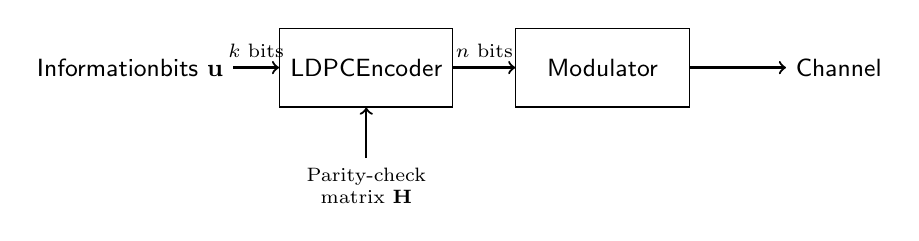
\begin{tikzpicture}[
  block/.style={rectangle, draw, minimum width=2.2cm, minimum height=1cm, font=\sffamily\small},
  node distance=2.5cm,
  font=\small
]
\node (input) {\sffamily Information\\bits $\mathbf{u}$};
\node[block, right of=input, node distance=3cm] (encoder) {LDPC\\Encoder};
\node[block, right of=encoder, node distance=3cm] (output_block) {Modulator};
\node[right of=output_block, node distance=3cm] (output) {\sffamily Channel};

\node[below of=encoder, node distance=1.5cm, font=\scriptsize, align=center] (matrix) {Parity-check\\matrix $\mathbf{H}$};

\draw[->,thick] (input) -- node[above,font=\scriptsize] {$k$ bits} (encoder);
\draw[->,thick] (encoder) -- node[above,font=\scriptsize] {$n$ bits} (output_block);
\draw[->,thick] (output_block) -- (output);
\draw[->,thick] (matrix) -- (encoder);
\end{tikzpicture}
\end{center}

\subsection{Decoder Block Diagram}

\begin{center}
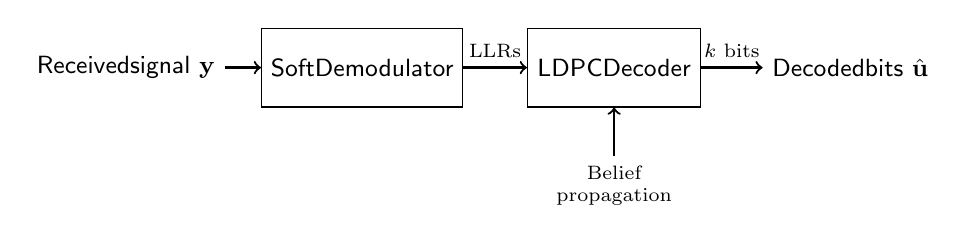
\begin{tikzpicture}[
  block/.style={rectangle, draw, minimum width=2.2cm, minimum height=1cm, font=\sffamily\small},
  node distance=2.5cm,
  font=\small
]
\node (input) {\sffamily Received\\signal $\mathbf{y}$};
\node[block, right of=input, node distance=3cm] (demod) {Soft\\Demodulator};
\node[block, right of=demod, node distance=3.2cm] (decoder) {LDPC\\Decoder};
\node[right of=decoder, node distance=3cm] (output) {\sffamily Decoded\\bits $\hat{\mathbf{u}}$};

\node[below of=decoder, node distance=1.5cm, font=\scriptsize, align=center] (matrix) {Belief\\propagation};

\draw[->,thick] (input) -- (demod);
\draw[->,thick] (demod) -- node[above,font=\scriptsize] {LLRs} (decoder);
\draw[->,thick] (decoder) -- node[above,font=\scriptsize] {$k$ bits} (output);
\draw[->,thick] (matrix) -- (decoder);
\end{tikzpicture}
\end{center}

\subsection{Belief Propagation Algorithm}

The LDPC decoder uses iterative message passing between variable and check nodes:

\textbf{Initialization:} For each received symbol $y_j$, compute log-likelihood ratio (LLR):
\begin{equation}
L_j = \ln\frac{P(c_j = 0 | y_j)}{P(c_j = 1 | y_j)} = \frac{2y_j}{\sigma^2}
\end{equation}
where:
\begin{itemize}
\item $L_j$ = initial LLR for bit $j$
\item $y_j$ = received soft value
\item $\sigma^2$ = noise variance
\item Positive $L_j$ indicates bit 0, negative indicates bit 1
\end{itemize}

\textbf{Check-to-Variable Messages:} Each check node sends messages to connected variable nodes:
\begin{equation}
m_{i \rightarrow j}^{(t)} = 2 \tanh^{-1}\left(\prod_{j' \in N(i) \setminus j} \tanh\left(\frac{m_{j' \rightarrow i}^{(t-1)}}{2}\right)\right)
\end{equation}
where:
\begin{itemize}
\item $m_{i \rightarrow j}^{(t)}$ = message from check $i$ to variable $j$ at iteration $t$
\item $N(i)$ = set of variable nodes connected to check node $i$
\item $\setminus j$ = excluding variable node $j$
\end{itemize}

\textbf{Variable-to-Check Messages:} Each variable node aggregates incoming messages:
\begin{equation}
m_{j \rightarrow i}^{(t)} = L_j + \sum_{i' \in M(j) \setminus i} m_{i' \rightarrow j}^{(t-1)}
\end{equation}
where:
\begin{itemize}
\item $M(j)$ = set of check nodes connected to variable node $j$
\item $L_j$ = channel LLR (from equation~10)
\end{itemize}

\textbf{Decision:} After $T$ iterations or convergence, compute final LLR:
\begin{equation}
L_j^{(T)} = L_j + \sum_{i \in M(j)} m_{i \rightarrow j}^{(T)}
\end{equation}
\begin{equation}
\hat{c}_j = \begin{cases}
0 & \text{if } L_j^{(T)} > 0 \\
1 & \text{if } L_j^{(T)} \leq 0
\end{cases}
\end{equation}

\begin{warningbox}
\textbf{Convergence is not guaranteed.} In low SNR conditions or with poor code design, the decoder may not converge to a valid codeword within the maximum iterations. Typical implementations use 50--100 iterations maximum.
\end{warningbox}

\subsection{Decoding Complexity}

The computational complexity per iteration is:
\begin{equation}
O(E) = O(n \cdot d_v) = O(m \cdot d_c)
\end{equation}
where:
\begin{itemize}
\item $E$ = number of edges in Tanner graph
\item $n \cdot d_v$ = total connections (variable node perspective)
\item $m \cdot d_c$ = total connections (check node perspective)
\item For sparse graphs: $E \ll n \cdot m$ (much less than dense codes)
\end{itemize}

\section{Performance Analysis}

\subsection{Bit Error Rate Performance}

The theoretical BER for LDPC codes in AWGN approaches the Shannon limit:
\begin{equation}
\mathrm{BER}_{\mathrm{LDPC}} \approx Q\left(\sqrt{2R \cdot \frac{E_b}{N_0}}\right) \quad \text{for } \frac{E_b}{N_0} > E_b/N_0^*
\end{equation}
where:
\begin{itemize}
\item $R$ = code rate
\item $E_b/N_0^*$ = threshold $E_b/N_0$ for waterfall region
\item $Q(x)$ = Gaussian Q-function
\end{itemize}

\textbf{Shannon limit for rate $R$:}
\begin{equation}
\frac{E_b}{N_0}\bigg|_{\text{Shannon}} = 2^{2R} - 1 \quad \text{(linear scale)}
\end{equation}

For rate $R = 1/2$: Shannon limit = 0~dB, typical LDPC achieves $\sim$0.5~dB.

\subsection{Performance Characteristics}

LDPC codes exhibit three distinct regions in their BER curves:

\begin{center}
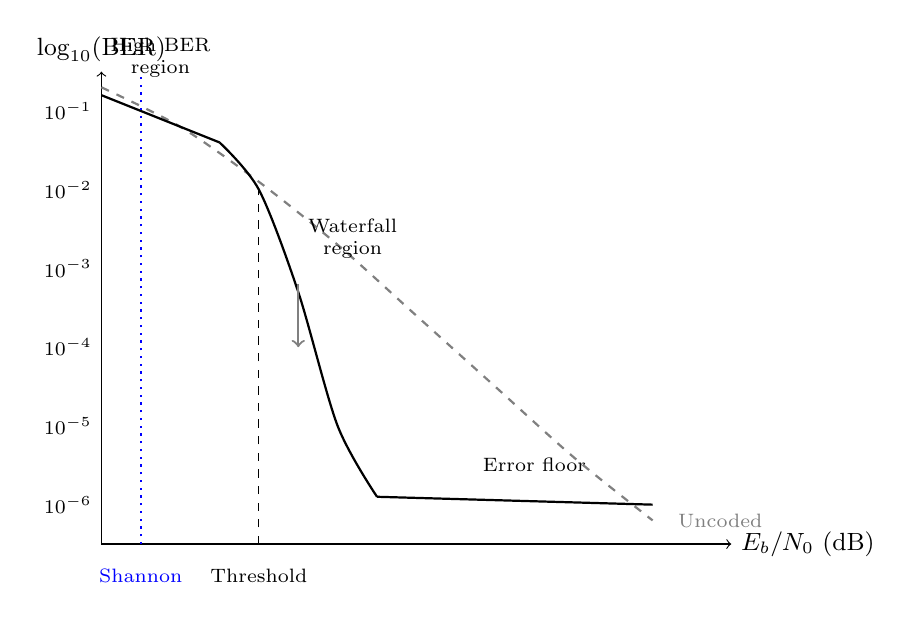
\begin{tikzpicture}[scale=1.0]
% Axes
\draw[->] (0,0) -- (8,0) node[right,font=\small] {$E_b/N_0$ (dB)};
\draw[->] (0,0) -- (0,6) node[above,font=\small] {$\log_{10}(\mathrm{BER})$};

% Y-axis labels
\node[left,font=\scriptsize] at (0,5.5) {$10^{-1}$};
\node[left,font=\scriptsize] at (0,4.5) {$10^{-2}$};
\node[left,font=\scriptsize] at (0,3.5) {$10^{-3}$};
\node[left,font=\scriptsize] at (0,2.5) {$10^{-4}$};
\node[left,font=\scriptsize] at (0,1.5) {$10^{-5}$};
\node[left,font=\scriptsize] at (0,0.5) {$10^{-6}$};

% Uncoded curve
\draw[thick,gray,dashed] plot[smooth] coordinates {(0,5.8) (1,5.3) (2,4.6) (3,3.8) (4,2.9) (5,2.0) (6,1.1) (7,0.3)};
\node[right,font=\scriptsize,gray] at (7.2,0.3) {Uncoded};

% LDPC curve with three regions
% High BER region
\draw[thick,black] plot[smooth] coordinates {(0,5.7) (0.5,5.5) (1,5.3) (1.5,5.1)};
\node[above,font=\scriptsize,align=center] at (0.75,5.8) {High BER\\region};

% Waterfall region (steep drop)
\draw[thick,black] plot[smooth] coordinates {(1.5,5.1) (2,4.5) (2.5,3.2) (3,1.5) (3.5,0.6)};
\node[above right,font=\scriptsize,align=center] at (2.5,3.5) {Waterfall\\region};
\draw[->,thick,gray] (2.5,3.3) -- (2.5,2.5);

% Error floor
\draw[thick,black] (3.5,0.6) -- (7,0.5);
\node[above,font=\scriptsize,align=center] at (5.5,0.8) {Error floor};

% Threshold marker
\draw[dashed,thin] (2,0) -- (2,4.5);
\node[below,font=\scriptsize] at (2,-0.2) {Threshold};

% Shannon limit marker
\draw[dotted,thick,blue] (0.5,0) -- (0.5,6);
\node[below,font=\scriptsize,blue] at (0.5,-0.2) {Shannon};
\end{tikzpicture}
\end{center}

\textbf{Region 1---High BER:} Below threshold, decoder does not converge effectively. Performance similar to uncoded transmission.

\textbf{Region 2---Waterfall:} At threshold $E_b/N_0$, BER drops rapidly (typically $10^{-1}$ to $10^{-5}$ over 1--2~dB). This is the characteristic LDPC performance region.

\textbf{Region 3---Error Floor:} At high $E_b/N_0$, BER flattens to a minimum value caused by:
\begin{itemize}
\item \textbf{Trapping sets:} Small subgraphs that cause decoder failures
\item \textbf{Finite block length:} Shorter codes have higher floors
\item \textbf{Decoder limitations:} Practical implementations have constraints
\end{itemize}

\subsection{Coding Gain}

The coding gain is the reduction in required $E_b/N_0$ to achieve a target BER:
\begin{equation}
G_c = \left(\frac{E_b}{N_0}\right)_{\text{uncoded}} - \left(\frac{E_b}{N_0}\right)_{\text{coded}} \quad \text{(dB)}
\end{equation}

\textbf{Example:} For BER $= 10^{-5}$:
\begin{center}
\begin{tabular}{@{}lrl@{}}
\toprule
Scheme & $E_b/N_0$ Required & Coding Gain \\
\midrule
Uncoded BPSK & 9.6~dB & --- \\
LDPC ($R=1/2$) & 1.0~dB & 8.6~dB \\
LDPC ($R=2/3$) & 2.5~dB & 7.1~dB \\
LDPC ($R=3/4$) & 3.2~dB & 6.4~dB \\
\bottomrule
\end{tabular}
\end{center}

\subsection{LDPC vs Other Forward Error Correction Codes}

\begin{center}
\begin{tabular}{@{}lcccc@{}}
\toprule
Code Type & Complexity & Performance & Latency & Flexibility \\
\midrule
Hamming & Low & Poor & Low & Low \\
Reed-Solomon & Medium & Good & Medium & Medium \\
Convolutional & Low & Good & Low & Low \\
Turbo & High & Excellent & High & Medium \\
\textbf{LDPC} & \textbf{Medium} & \textbf{Excellent} & \textbf{Medium} & \textbf{High} \\
Polar & Medium & Excellent & Low & High \\
\bottomrule
\end{tabular}
\end{center}

\begin{keyconcept}
LDPC codes offer the \textbf{best trade-off} between performance, complexity, and flexibility. While Turbo codes offer similar performance, LDPC codes have lower latency and are easier to parallelize in hardware, making them the preferred choice for modern high-speed systems.
\end{keyconcept}

\section{Worked Example: DVB-S2 Satellite Link}

\textbf{Scenario:} Design an LDPC-coded satellite downlink for digital video broadcasting.

\subsection*{Given Parameters}

\begin{tabular}{@{}ll@{}}
Code rate & $R = 3/4$ \\
Block length & $n = 64{,}800$ bits \\
Information bits & $k = 48{,}600$ bits \\
Modulation & QPSK \\
Symbol rate & $R_s = 27.5$~Msym/s \\
Channel & AWGN with $E_b/N_0 = 4.0$~dB \\
Target BER & $10^{-7}$ (after FEC) \\
\end{tabular}

\subsection*{Step 1: Calculate Bit Rate}

For QPSK, each symbol carries 2 bits:
\begin{equation}
R_b = R_s \times \log_2(M) \times R = 27.5 \times 2 \times \frac{3}{4} = 41.25~\text{Mbps}
\end{equation}

\subsection*{Step 2: Uncoded BER}

Without LDPC, QPSK in AWGN gives:
\begin{equation}
\mathrm{BER}_{\text{uncoded}} = Q\left(\sqrt{\frac{2E_b}{N_0}}\right) = Q(\sqrt{2 \times 10^{0.4}}) \approx 1.25 \times 10^{-2}
\end{equation}

\textbf{Result:} 1.25\% bit errors---completely unusable for video!

\subsection*{Step 3: LDPC Decoding Threshold}

For DVB-S2 LDPC $(n=64800, R=3/4)$, the waterfall threshold is approximately:
\begin{equation}
\left(\frac{E_b}{N_0}\right)_{\text{threshold}} \approx 3.0~\text{dB}
\end{equation}

Since our $E_b/N_0 = 4.0$~dB $>$ 3.0~dB, we are in the waterfall region.

\subsection*{Step 4: LDPC-Coded BER}

The DVB-S2 LDPC code achieves at $E_b/N_0 = 4.0$~dB:
\begin{equation}
\mathrm{BER}_{\text{coded}} \approx 10^{-8}
\end{equation}

\textbf{Result:} Exceeds target BER of $10^{-7}$ with margin!

\subsection*{Step 5: Coding Gain Calculation}

To achieve BER $= 10^{-7}$ uncoded requires $E_b/N_0 \approx 11.3$~dB (from Q-function).

\begin{equation}
G_c = 11.3 - 4.0 = 7.3~\text{dB coding gain}
\end{equation}

\begin{calloutbox}[colback=black!8!white,colframe=black]{Link Budget Summary}
\textbf{Result: LDPC enables reliable DVB-S2 transmission}

The 7.3~dB coding gain means:
\begin{itemize}
\item \textbf{Smaller antennas:} Can use 60~cm dish instead of 1.5~m
\item \textbf{Lower power:} Satellite can transmit 5$\times$ less power
\item \textbf{Higher throughput:} 41.25~Mbps enables HD video streams
\end{itemize}

\textbf{Decoding latency:} With typical 35 iterations at 27.5~Msym/s, decoding adds $\sim$2.4~ms latency---acceptable for broadcast video.
\end{calloutbox}

\section{Practical Applications}

\subsection{Digital Video Broadcasting (DVB-S2/S2X)}

Satellite television and data broadcasting:
\begin{itemize}
\item \textbf{Standard:} DVB-S2 (2005), DVB-S2X (2014)
\item \textbf{Code rates:} 1/4, 1/3, 2/5, 1/2, 3/5, 2/3, 3/4, 4/5, 5/6, 8/9, 9/10
\item \textbf{Block lengths:} 16,200 bits (short) or 64,800 bits (normal)
\item \textbf{Modulation:} QPSK, 8PSK, 16APSK, 32APSK
\item \textbf{Performance:} Within 0.7--1.0~dB of Shannon limit
\item \textbf{Applications:} Satellite TV, satellite internet, VSAT networks
\end{itemize}

\subsection{WiFi (IEEE 802.11n/ac/ax/be)}

Wireless local area networks:
\begin{itemize}
\item \textbf{802.11n (2009):} Optional LDPC support
\item \textbf{802.11ac (2013):} LDPC mandatory for 256-QAM
\item \textbf{802.11ax (Wi-Fi 6, 2019):} Enhanced LDPC for improved range
\item \textbf{802.11be (Wi-Fi 7, 2024):} LDPC for up to 4096-QAM
\item \textbf{Code rates:} 1/2, 2/3, 3/4, 5/6
\item \textbf{Block lengths:} 648, 1296, 1944 bits
\item \textbf{Benefit:} 2--3~dB gain enables higher data rates and extended range
\end{itemize}

\subsection{5G New Radio (3GPP NR)}

Fifth-generation cellular networks:
\begin{itemize}
\item \textbf{Standard:} 3GPP Release 15+ (2018)
\item \textbf{Usage:} Data channels (eMBB, URLLC)
\item \textbf{Code rates:} $R = k/n$ with flexible $k$, $n$
\item \textbf{Block lengths:} Up to 8448 bits
\item \textbf{Base graphs:} Two optimized structures (BG1, BG2)
\item \textbf{Advantage over Turbo:} Lower latency, better parallelization
\item \textbf{Performance:} Enables multi-Gbps peak rates
\end{itemize}

\subsection{Solid-State Drives (SSDs)}

Flash memory error correction:
\begin{itemize}
\item \textbf{Application:} Protect against bit flips in NAND flash
\item \textbf{Challenge:} Error rate increases with flash wear (P/E cycles)
\item \textbf{Code rates:} Adaptive based on flash condition
\item \textbf{LDPC advantage:} Can correct 100+ errors per 4~KB page
\item \textbf{Implementations:} Controller-based hardware decoders
\item \textbf{Impact:} Enables higher density (TLC, QLC flash) and longer endurance
\end{itemize}

\subsection{Deep-Space Communications}

NASA/ESA interplanetary missions:
\begin{itemize}
\item \textbf{Standard:} CCSDS (Consultative Committee for Space Data Systems)
\item \textbf{Missions:} Mars rovers, Voyager extended mission, BepiColombo
\item \textbf{Code rates:} 1/2, 2/3, 4/5
\item \textbf{Concatenation:} Often paired with Reed-Solomon outer code
\item \textbf{Benefit:} Maximize data return from extreme path loss ($>$200~dB)
\end{itemize}

\subsection{LDPC in Chimera}

The Chimera modem uses LDPC for acoustic underwater communications:
\begin{itemize}
\item \textbf{Library:} \texttt{chimera-core} Rust implementation
\item \textbf{Decoder:} Iterative belief propagation with LLRs
\item \textbf{Max iterations:} Configurable (typically 50)
\item \textbf{Code rates:} 1/2, 2/3, 3/4 (preset-dependent)
\item \textbf{Block lengths:} 576 to 1944 bits
\item \textbf{Performance metrics:} Pre-FEC BER, Post-FEC BER, iteration count, frame failures
\end{itemize}

\section{Advantages and Disadvantages}

\subsection{Advantages}

\begin{itemize}
\item \textbf{Near-Shannon-limit performance:} Within 0.5~dB of theoretical capacity
\item \textbf{Flexible code rates:} Easily adapted from 1/4 to 9/10
\item \textbf{Parallel decoding:} Sparse graph enables efficient hardware implementation
\item \textbf{Soft-decision decoding:} Effectively uses LLR information from demodulator
\item \textbf{Scalable block lengths:} Works from 576 to 64,800+ bits
\item \textbf{Low latency:} Faster convergence than Turbo codes
\item \textbf{Standardized:} Adopted in DVB-S2, 802.11n/ac/ax, 5G NR, CCSDS
\end{itemize}

\subsection{Disadvantages}

\begin{itemize}
\item \textbf{Encoding complexity:} Requires matrix operations (higher than convolutional codes)
\item \textbf{Error floor:} Does not eliminate all errors at high SNR
\item \textbf{Latency:} Iterative decoding adds delay (typically 20--50 iterations)
\item \textbf{Memory requirements:} Storing parity-check matrix and messages
\item \textbf{Design complexity:} Optimizing degree distribution requires expertise
\item \textbf{Variable decoding time:} Convergence speed depends on channel conditions
\end{itemize}

\section{Summary}

\begin{center}
\begin{tabular}{@{}ll@{}}
\toprule
\textbf{Aspect} & \textbf{LDPC Codes} \\
\midrule
Invention & Robert Gallager (MIT, 1962) \\
Key property & Sparse parity-check matrix \\
Decoding algorithm & Iterative belief propagation \\
Performance & Within 0.5~dB of Shannon limit \\
Code rates & 1/4 to 9/10 (highly flexible) \\
Block lengths & 576 to 64,800+ bits \\
Complexity & Medium (sparse graph operations) \\
Latency & Medium (20--50 iterations typical) \\
Standards & DVB-S2, WiFi 5/6/7, 5G NR, SSDs \\
Best for & High-throughput, near-capacity systems \\
\bottomrule
\end{tabular}
\end{center}

\begin{keyconcept}
LDPC codes represent the \textbf{state-of-the-art in practical error correction}. Their combination of near-optimal performance, flexible design, and efficient hardware implementation has made them the dominant FEC choice in modern wireless, satellite, and storage systems.
\end{keyconcept}

\section{Further Reading}

\textbf{Related chapters in this book:}
\begin{itemize}
\item Chapter~\ref{ch:fec}: Forward Error Correction---general FEC concepts and comparison
\item Chapter~\ref{ch:ber}: Bit Error Rate---understanding error metrics
\item Chapter~\ref{ch:awgn}: AWGN Channel Model---the canonical test channel
\item Chapter~\ref{ch:qpsk}: QPSK Modulation---often paired with LDPC in practice
\item Chapter~\ref{ch:shannon}: Shannon's Theorem---theoretical capacity limits
\end{itemize}

\textbf{Foundational papers:}
\begin{itemize}
\item Gallager, R.G. (1962). ``Low-Density Parity-Check Codes.'' IRE Transactions on Information Theory.
\item MacKay, D.J.C. and Neal, R.M. (1996). ``Near Shannon limit performance of low density parity check codes.''
\item Richardson, T.J. and Urbanke, R.L. (2001). ``The capacity of low-density parity-check codes under message-passing decoding.''
\end{itemize}

\textbf{Standards documents:}
\begin{itemize}
\item ETSI EN 302 307: ``DVB-S2 Digital Video Broadcasting''
\item IEEE 802.11n/ac/ax: ``Wireless LAN Medium Access Control (MAC) and Physical Layer (PHY)''
\item 3GPP TS 38.212: ``NR Multiplexing and channel coding''
\item CCSDS 131.0-B-3: ``Low Density Parity Check Codes for Use in Near-Earth and Deep Space Applications''
\end{itemize}
